\documentclass{LabReport}
\title{操作系统实验报告PA6}
\author{221900180 田永铭}
\date{\today}
\addbibresource{refs.bib}
\Chead{操作系统实验报告PA6 221900180 田永铭}
\Cfoot{\thepage}
\usepackage{listings}
\usepackage{graphicx} 
\usepackage{tikzsymbols}
\usepackage{tikz}
\usepackage{hyperref}

\begin{document}
	\maketitle
	
	\tableofcontents
	
	\newpage
	
	\section{实验要求}
使用C语言和pthread线程库实现一个多线程的采用蒙特卡洛随机采样算法计算π值的程序。\\
具体要求:\\
1)程序需要支持命令行参数-t,用于指定程序运行时创建多少个线程用于计算;\\
2)了解GCC标准库提供的随机函数的实现,分析其如何保证多线程安全,以及对多线程程序性能的影响;\\
3)需结合自身硬件环境(如CPU核心数),分析同等总采样次数的情况下,不同的线程数,程序的运行时间开销,并分析原因。

	\section{实验环境}
	
	\begin{itemize}
		\item 操作系统:wsl2
		\item 编程语言:C语言,python
		\item 使用工具:makefile编译;python绘图的包等
		\item 虚拟系统版本:Ubuntu-22.04
	\end{itemize}
	
	\section{实验原理}
	\begin{itemize}
		\item \textbf{蒙特卡洛采样求$\pi$的原理:}
		\par\hspace{2em}
		蒙特卡洛方法是一种通过随机抽样进行数值计算的方法。在计算$\pi$值时,我们可以利用以下几何概率的方法(注意我仅仅使用了第一象限来计算):\par\hspace{2em}
		在一个边长为1的正方形内随机生成点,以正方形左下角的点为圆心,以1为半径画一个圆,圆的面积为$\pi$/4,正方形的面积为4/4。\par\hspace{2em}
		随机生成点(x, y),其中x和y的范围在[0, 1]之间, 并判断点是否在圆内,即判断$x^2 + y^2 \leq 1$。\par\hspace{2em}
		统计在圆内的点数和总点数的比例,该比例约等于圆面积与正方形面积之比,即$\pi / 4$。\par\hspace{2em}
		通过此比例估算$\pi$值,即$\pi \approx 4 \times (\text{圆内点数} / \text{总点数})$。
		
		\item \textbf{多线程并发的原理:} \par\hspace{2em}使用多线程可以并行执行任务,减少程序运行时间。 \par\hspace{2em}
		将总采样点数分配给多个线程,每个线程独立进行随机采样,计算自己采样点中落在圆内的点数。主线程收集所有子线程的计算结果,汇总得到最终的π值估算。
		\item \textbf{保护多线程正确的原理:}
		\par\hspace{2em}
		采用pthread库;采用加互斥锁的方法使得修改共享变量是安全的;标准C库提供的rand()函数在多线程环境中不是线程安全的,应当使用rand\_r()函数;以此保护多线程正确。
		
		\item \textbf{实验结果可视化原理:}
		\par\hspace{2em}利用python语言格式化了输出,并且调用matplotlib.pyplot包来进行绘图。
		
	\end{itemize}
	
	\section{实验过程}
	\par\hspace{0em}实验主要分为以下几个步骤:
	
	\begin{enumerate}
		\item 实现单线程MC算法求$\pi$值
		\item 实现多线程MC算法求$\pi$值
		\item 提供使用-t来传线程数的服务
		\item 编写makefile,方便运行
		\item 实现格式化输出和绘图代码
		\item 展示文件结构
	\end{enumerate}
	
	\subsection{实现单线程MC算法求$\pi$值}
	根据实验原理部分的介绍,可以简单地实现出单线程MC算法,核心代码如下:
\begin{lstlisting}[language=python,frame=shadowbox]
#define TOTAL_POINTS 10080000

int thread_nums = 1; // 进行实验的线程数
int points_in_circle_nums = 0; //落入圆内的总点数
double pi = 0; //pi的计算值

void *sampling()
{
	int cnt = 0;
	unsigned int seed = (unsigned int)time(NULL); //定义时间种子
	
	for (int i = 0; i < TOTAL_POINTS; i++)
	{
		double x = (double)rand_r(&seed) / RAND_MAX;
		double y = (double)rand_r(&seed) / RAND_MAX;
		if (x * x + y * y <= 1) cnt++; //落在圆内,则cnt++
	}
	points_in_circle_nums += cnt;
	return (void *)0;
}

int main(int argc, char *argv[])
{
	//计算pi
	pi = 4.0 * points_in_circle_nums / TOTAL_POINTS;
	//打印结果
	printf("总点数的值: %d\n", TOTAL_POINTS);
	printf("落在圆内的总点数的值: %d\n", points_in_circle_nums);
	printf("计算得到的π的值: %lf\n", pi);
	return 0;
}
\end{lstlisting}
	此部分非常简单,不再赘述。
	
	\subsection{实现多线程MC算法求$\pi$值}
	我的方法是:将TOTAL\_POINTS这么多个采样点均分给n个线程一起来采样,它们各自统计落在圆内的点数,统计完成后利用加锁处理将这个值加到落在圆内的总点数变量上。实现如下:\\
	首先引入 <unistd.h><pthread.h><stdlib.h>等相关多线程的库。\\
	然后是创线程,分配线程号,销毁线程的操作,代码如下:
	
	\begin{lstlisting}[language=python,frame=shadowbox]
//分配线程号,用于传参
pthread_t threads[MAX_THREAD_NUMS];
int threadsId[MAX_THREAD_NUMS];
for (int i = 0; i < MAX_THREAD_NUMS; i++) threadsId[i] = i;

//创线程
for (int i = 0; i < thread_nums; i++) pthread_create(&threads[i], NULL, sampling, &threadsId[i]);

//销线程
for (int i = 0; i < thread_nums; i++) pthread_join(threads[i], NULL);
	\end{lstlisting}
	
	再接着需要加锁来保护并发,同时传参(线程号)给采样函数sampling,代码如下:
	
	\begin{lstlisting}[language=python,frame=shadowbox]
pthread_mutex_t mutex = PTHREAD_MUTEX_INITIALIZER; // 定义互斥锁		

void *sampling(void *arg)
{
	//获取线程id
	int *id = (int *)arg;
	//统计该线程计算得到的落入圆内的点数
	int cnt = 0;
	unsigned int seed = (unsigned int)time(NULL); //定义时间种子
	
	//一共采样nums_of_points_to_sample_of_each_thread个
	for (int i = 0; i < nums_of_points_to_sample_of_each_thread; i++)
	{
		// 一定不能用rand,应该用rand_r!!!
		double x = (double)rand_r(&seed) / RAND_MAX;
		double y = (double)rand_r(&seed) / RAND_MAX;
		if (x * x + y * y <= 1) cnt++; //落在圆内,则cnt++
	}
	//由于多线程要对全局变量points_in_circle_nums修改,要上互斥锁保护一下
	pthread_mutex_lock(&mutex);
	points_in_circle_nums += cnt;
	pthread_mutex_unlock(&mutex);
	return (void *)0;
}

pthread_mutex_destroy(&mutex); // 销毁互斥锁
	\end{lstlisting}
	
	由此便实现了多线程MC求$\pi$值的算法。
	
	\subsection{提供使用-t来传线程数的服务}
	
		\begin{lstlisting}[language=python,frame=shadowbox]
int main(int argc, char *argv[])
{
	//如果没使用-t传参
	if(argc == 1) thread_nums = 1;
	//如果使用了-t传参
	else if (argc != 3 || argv[1][0] != '-' || argv[1][1] != 't')
	{
		printf("grammer fault!\n");
		return 1;
	}
	else
	{
		if (thread_nums = atoi(argv[2])) {}
		else
		{
			printf("argument invalid!\n");
			return 1;
		}
	}
	\end{lstlisting}
	
	通过这样的处理,使得编译运行时支持"./main -t 4"类似的服务。同时,我也注意了异常的处理。
	
	\subsection{编写makefile,方便运行}
	我编写了makefile,来使得可以用``make"来编译,使用``make output"命令一下运行7个结果到指定位置,使用``make clear"来清除main文件。
	\begin{lstlisting}[language=python,frame=shadowbox]
all:
	gcc -lpthread -o main ./multi_thread_calculate_pi_MC.c
output: 
	./main -t 1 > ./result/output/test_thread=1.out
	./main -t 2 > ./result/output/test_thread=2.out
	./main -t 4 > ./result/output/test_thread=4.out
	./main -t 8 > ./result/output/test_thread=8.out
	./main -t 16 > ./result/output/test_thread=16.out
	./main -t 32 > ./result/output/test_thread=32.out
	./main -t 64 > ./result/output/test_thread=64.out
clear:
	rm -f main
	\end{lstlisting}
	
	\subsection{实现格式化输出和绘图代码}
	由于我在c文件中利用clock()统计的时间不太准,也不能方便地绘图。所以我单独用一个python文件plot.py来进行格式化输出与程序运行时间的统计和绘制。核心代码大体如下:
		\begin{lstlisting}[language=python,frame=shadowbox]
# 运行5次可执行文件并记录时间
for exe in executables:
	for arg in args:
		times = []
		for _ in range(5):  # 对每个参数运行5次
			start = time.time()
			subprocess.run([f"./{exe}", "-t", str(arg)])
			end = time.time()
			times.append(end - start)
		results[exe][arg] = times

# 将数据写入文件
with open('./running_time.txt', 'w') as file:
	for exe in executables:
		for arg in args:
			for time_val in results[exe][arg]:
				file.write(f"{exe} {arg} {time_val}\n")
				
......(省略打开文件,求中位数等等代码)

# 绘图
plt.figure(figsize=(10, 6))
for exe in results:
	args = list(results[exe].keys())
	plt.errorbar(args, medians[exe], 
	yerr=errors[exe], capsize=5, label=exe)

plt.xlabel('Numbers of threads')
plt.ylabel('Time (s)')
plt.title('Execution time of different numbers of threads')
plt.xticks(args)
plt.legend()
plt.grid(True)
plt.savefig(f'./result/img/exeTime_{time.time()}.png')
plt.clf()
	\end{lstlisting}
	由此,我能够通过运行``python plot.py"来获取结果并绘制运行时间随着线程数量的变化图。
	
	\subsection{展示文件结构}
	最终我的文件结构如下:
	
\begin{figure}[h!]
	\centering
	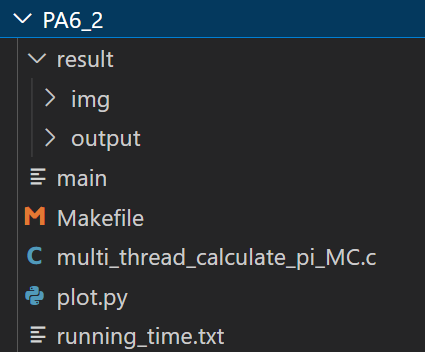
\includegraphics[width=0.7\linewidth]{figures/file_structure}
	\caption{filestructure}
	\label{fig:filestructure}
\end{figure}
	其中,c文件为核心代码文件,py文件是绘图文件,用py文件跑代码生成的结果在result里面,分为图片img和输出output,makefile用来编译代码。

	\section{实验结果汇报}
	为方便助教批改,我按照要求依次汇报,当然首先简要展示一些计算$\pi$的结果,而计算时间的分析和多线程的分析跟在后面展示。
	\subsection{展示计算$\pi$的结果}
	采用不同线程数对计算$\pi$的结果影响不大,而蒙特卡洛采样的总的点数的数目对计算结果影响较大,数目越多越准,但是计算耗时也越长,综合考量,我选取的是10080000这个数字,它刚好能被1到10的数字整除,也能被16、32和64整除。这边很简单,就不一一对比,展示一下大致计算的$\pi$数值,如下图所示:
	
\begin{figure}[h!]
	\centering
	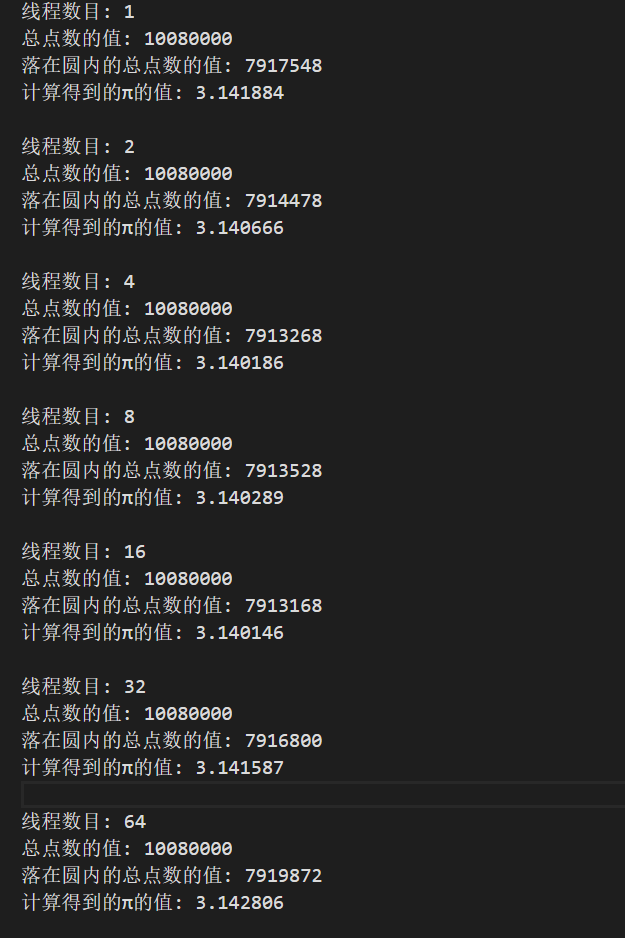
\includegraphics[width=0.5\linewidth]{figures/output_of_pi}
	\caption{outputofpi}
	\label{fig:outputofpi}
\end{figure}

	可见,结果大致具有四位有效数字,已经取得不错效果,并且采用不同数目线程计算得到的结果相差不大。
	
	\subsection{程序需要支持命令行参数-t}
	这部分代码已经在前面展示,下面演示输入命令``./main -t 5"的结果。
	
\begin{figure}[h!]
	\centering
	\includegraphics[width=0.7\linewidth]{"figures/-t 5"}
	\caption{-t-5}
	\label{fig:-t-5}
\end{figure}
	而输入的格式不合法的时候,也会打印不合法信息,因为我做了异常处理,此处不再展示。由此可见我的程序成功支持了命令行参数-t。
	
	\subsection{了解GCC标准库提供的随机函数的实现,分析多线程程序性能的影响}
	这一部分我首先踩了一个坑,就是我一开始利用GCC的rand()函数来实现多线程中的随机函数,导致我产生了如下的运行时间结果图:
	
\begin{figure}[h!]
	\centering
	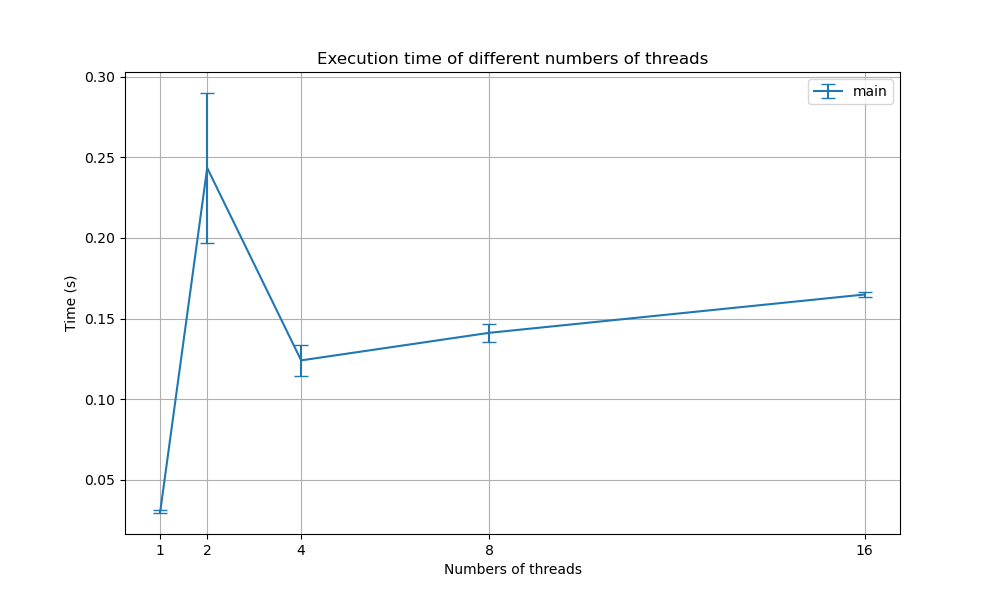
\includegraphics[width=1\linewidth]{figures/GccRand_power(2,i)threads}
	\caption{gccrandpower2ithreads}
	\label{fig:gccrandpower2ithreads}
\end{figure}
	
	这个结果出人意料之外,不在情理之中。经过和老师交流讨论以及查阅参考文献\href{https://www.jb51.net/article/232332.htm}{\color{blue} C语言中的rand()和rand\_r()详解},我发现不应该用rand(),正因为rand()不适合多线程,而rand\_r才是多线程适合的。具体原因如下\par
	\hspace{0em}对于上述蒙特卡洛法估计 $\pi$ 的程序,需要调用很多次rand(),由于GCC对rand()的实现为了保证多线程安全,需要每个线程频繁地对临界区进行上锁和解锁,而临界段被上锁后,其他线程无法完成rand()的调用从而被阻塞,这样会导致效率十分低下,因此会出现使用多线程反而程序运行更慢的问题,这多多线程程序的性能有很大的阻碍。\par
	\hspace{0em}改用rand\_r()后,GCC的实现中就不再需要上锁,也没有临界区,每个线程生成了它自己独有的随机数生成器,从而解决了多线程运行时所需要的时间反而更长这个问题,下面为使用rand\_r()产生的正确的结果:
	
\begin{figure}[h!]
	\centering
	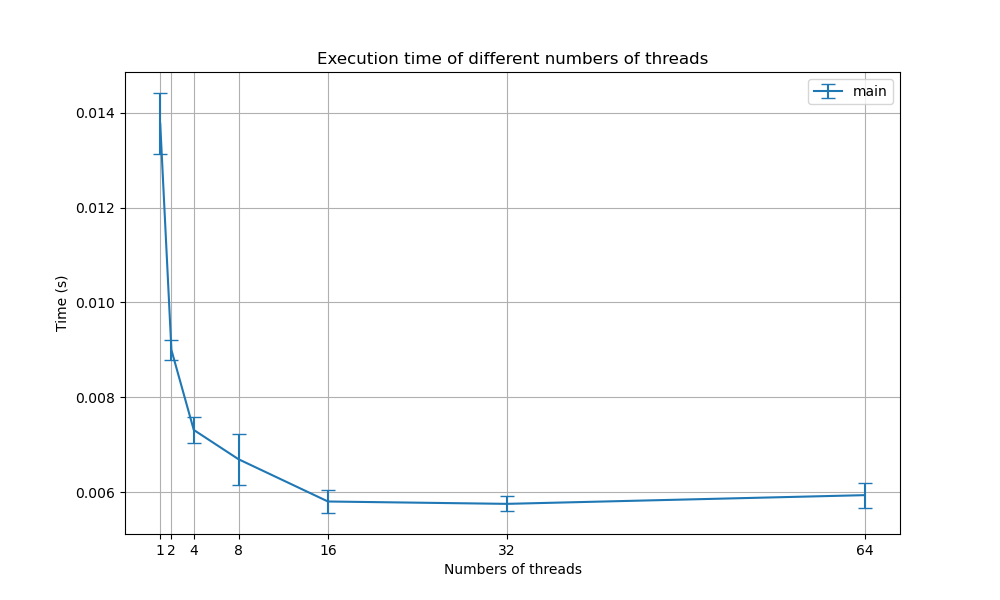
\includegraphics[width=1\linewidth]{figures/GccRandr_power(2,i)threads}
	\caption{gccrandrpower2ithreads}
	\label{fig:gccrandrpower2ithreads}
\end{figure}

	当然,一开始我没有发现这个问题,但是我知道问题可能出在随机数影响了效率,所以我自己写了个伪随机数,代码如下:
	
	\begin{lstlisting}[language=python,frame=shadowbox]
unsigned int myrand(unsigned int *seed)
	 {
		return (*seed) = ((((*seed) * 
			1103515245) + 12345) & 0xffffffff);
	 }
	 //后面将数字限制到0到1上除以的除数相应改为0xffffffff
	\end{lstlisting}
	
	得到了类似结果:\\\\\\\\
	
\begin{figure}[h!]
	\centering
	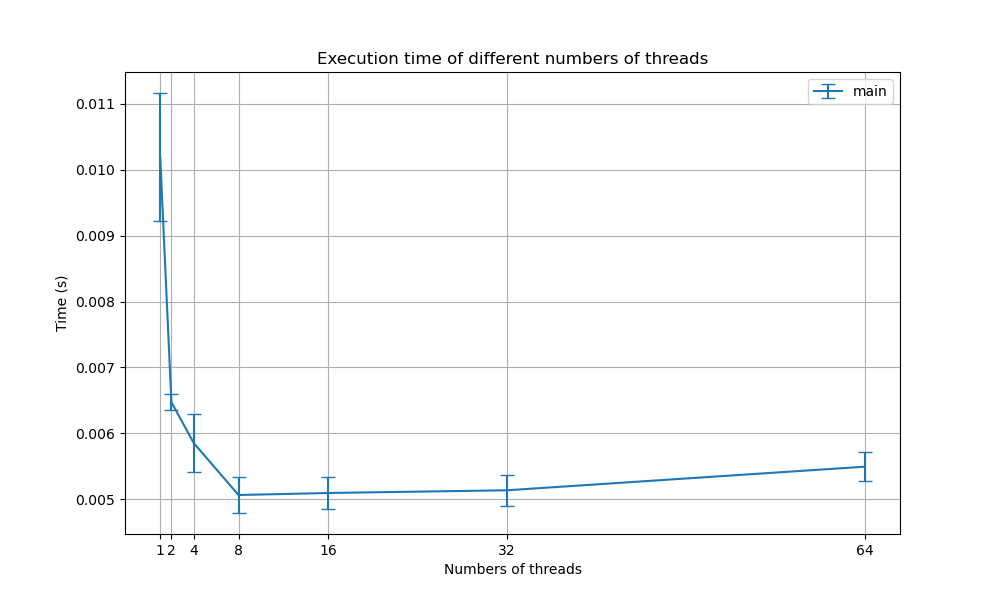
\includegraphics[width=0.8\linewidth]{figures/MyRand_power(2,i)threads_1008000points}
	\caption{myrandpower2ithreads}
	\label{fig:myrandpower2ithreads}
\end{figure}

	更进一步,增加线程种类数得到更精确的结果如下:
	
\begin{figure}[h!]
	\centering
	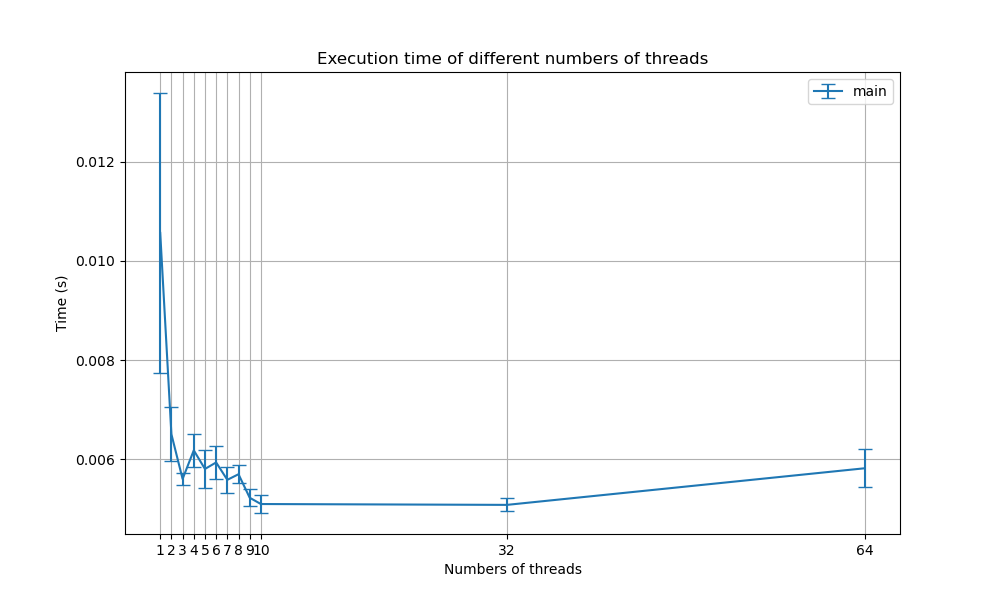
\includegraphics[width=0.8\linewidth]{figures/MyRand_MoreKindsOfThreads}
	\caption{myrandmorekindsofthreads}
	\label{fig:myrandmorekindsofthreads}
\end{figure}
	
	观察如上结果,处理错误的使用rand()产生的结果,其他的结果对于同样的总的采样点,都是一开始随着线程数增加程序运行时间逐渐减少,然后减少到一定程度又略微上升,但是仍然比单线程要块不少。\par\hspace{0em}具体解释如下:\par\hspace{0em}
	一开始线程数目比较少的情况下,随着线程数的增加,程序运行效率变高。这是因为蒙特卡洛采样程序是一个计算密集型的程序,需要大量使用CPU,而线程的增多使得多个CPU能同时运行程序,CPU的利用率变高,程序的运行速度加快。而随着线程数增加到一定程度时,为保护线程安全的互斥锁的使用增多,对线程的阻塞时间变多;同时,调度很多线程的开销也增大了,这又会导致程序运行效率的下降。\par\hspace{0em}
	综合以上两大方面的因素,使得结果呈现上面图片的形式,这是和理论非常符合的。
	
	\subsection{需结合自身硬件,分析不同的线程数程序的运行时间开销}
	其实这部分内容我在上一个部分{\color{red} ``分析多线程程序性能的影响"}已经{\color{red} 完全}报告完了。不过还可以简单再玩一下,做个bonus。由于taskset指令可以限制CPU的个数,所以我用这个指令再试一试。(这里补充一点,我的CPU有12核)\\
	
	运行命令 ``taskset -c 0 ./main"可以限制只有一个CPU,同理,``taskset -c 0,1 ./main"限制两个CPU,依次类推。我采用同一个总的采样数,同样使用4个线程,分别限制CPU个数从1到4个来做实验,采用``time"指令获取程序运行时间,运行时间如下图所示:
		
\begin{figure}[h!]
	\centering
	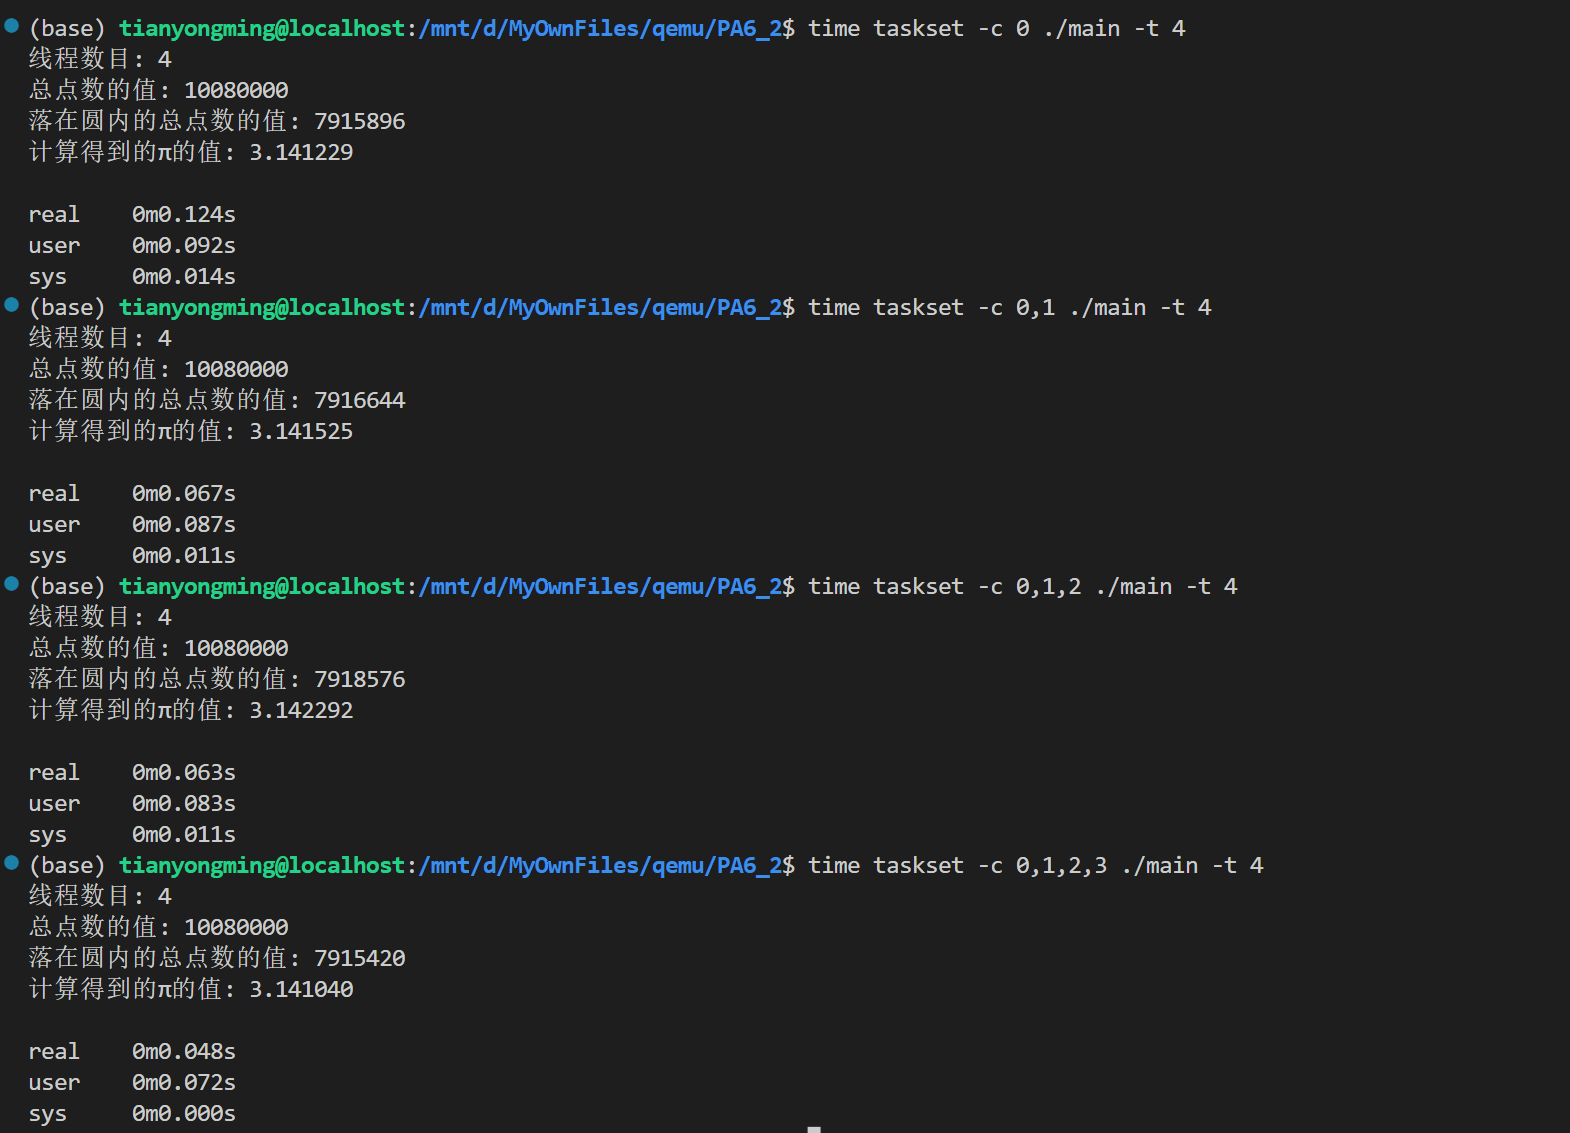
\includegraphics[width=0.7\linewidth]{figures/taskset}
	\caption{}
	\label{fig:taskset}
\end{figure}
	
	由此可见,CPU使用多少对程序的运行效率有显著的影响。而多线程之所以能在线程数目不太大的时候提高程序运行效率,就是因为上一部分所说的多CPU对程序运行效率的提升幅度大于为维护多线程采用锁和调度对程序运行效率的下降幅度。
	
	\section{总结与反思}
	\begin{itemize}
		\item 关于这次实验中我遇到的问题,确实并不多,主要体现在错误的使用rand(),以及绘图代码编写上的一点小bug。其他参考了老师发的pthread文献,学习了之后都非常容易实现,所以并不具体展开一个部分介绍我遇到的问题。而在实验中的各种探索我已经详尽的展示到上一部分之中。
		\item 这个程序其实和老师上课演示的很多并发程序比较相似,我找到了其中的连接点,比较轻松地实现了这次实验。
		\item 通过本次实验,我亲手实现了多线程的蒙特卡洛求圆周率值程序,进一步学习了pthread、mutex锁等等的使用,对多线程并发编程有了更深的理解。
	\end{itemize}

	\section{其它参考文献}
	除了正文给出的参考文献,我参考的文献仅有老师发的pthread教程。
	
\end{document}
